\documentclass[a4paper,11pt]{amsart}
\usepackage{graphicx,color}
\usepackage{codehighlight}
\usepackage{amssymb}
\usepackage{amsmath}


\long\def\COMMENT#1{\par\vbox{\hrule\vskip1pt \hrule width.125in height0ex #1\vskip1pt\hrule}}

\newcommand\cond{\operatorname{cond}}

\newtheorem{example}{Example}[section]
\newtheorem{exercise}{Exercise}[section]
\newtheorem{definition}{Definition}[section]




\title{Iterative methods}
\begin{document}
%\tableofcontents
%\COMMENT{
%Need vector norms and the definition of the corresponding
%matrix norm}


\section{Introduction}
This chapter concerns the numerical solution of linear systems,
\[
A u =  b,
\]
where the linear system comes from discretization of PDEs. Such
linear systems are characterized by being large, that
is $A$ is typically a $n\times n$ matrix where $n$ is
between $10^6$ to $10^9$. Furthermore, the matrix is typically
extremely sparse, typically containing only $\mathcal{O}(n)$ non-zeros.
However, $A^{-1}$ will typically full.
Finally, because the matrix is a discretized differential operator, the
condition number is typically large, and the condition number increases
as we increase the mesh resolution.  Because of these special characteristics,
special considerations needed in the choice of linear solver.
The difference between some different algorithms are illustrated in the following example.

\begin{example}[CPU times of different algorithms] 
\label{ex1}
In this example we will solve the problem
\begin{eqnarray*}
u - \Delta u &=& f,  \\
\frac{\partial u}{\partial n} &=& 0,
\end{eqnarray*}
on the unit square with first order Lagrange elements.
The problem is solved with four different methods:
\begin{itemize}
\item a LU solver,
\item Conjugate Gradient method,
\item Conjugate Gradient method with an ILU preconditioner,
\item Conjugate Gradient method with an AMG preconditioner.
\end{itemize}

Figure \ref{fig:cpu} shows that there is a dramatic difference between the different algorithms.
In fact, the Conjugate gradient (CG) with an AMG preconditioner is 22 times faster than the
slowest method, which is the CG solver without preconditioner.
However, the log-log plot reveals that all algorithms appears to have polynomial complexity,
i.e., $\mathcal{O}(N^\beta)$, with respect to number of degrees of freedom, $N$. The order
of the polynomial $\beta$ vary, though.


\begin{figure}[h]
\begin{center}
\label{fig:cpu}
\includegraphics[width=6cm]{../pics/cpu_plot.png}
\includegraphics[width=6cm]{../pics/log_cpu_plot.png}
\caption{The left figure shows the CPU time (in seconds) used to solve the linear system with
different mesh resolutions $(N,N)$. The right figure shows a log-log plot of the same data.}
\end{center}
\end{figure}


The code used in this experiment is as follows: 
\begin{python}
import time
from dolfin import *
lu_time = []
cg_time = []
cgilu_time = []
cgamg_time = []
Ns = []

parameters["krylov_solver"]["relative_tolerance"] = 1.0e-8
parameters["krylov_solver"]["absolute_tolerance"] = 1.0e-8
parameters["krylov_solver"]["monitor_convergence"] = True
parameters["krylov_solver"]["report"] = True
parameters["krylov_solver"]["maximum_iterations"] = 50000

for N in [32, 64, 128, 256, 512, 1024]:

  Ns.append(N)

  mesh = UnitSquare(N, N)
  print " N ", N, " dofs ", mesh.num_vertices()
  V = FunctionSpace(mesh, "Lagrange", 1)
  u = TrialFunction(V)
  v = TestFunction(V)

  f = Expression("sin(x[0]*12) - x[1]")
  a = u*v*dx  + inner(grad(u), grad(v))*dx
  L = f*v*dx

  U = Function(V)

  A = assemble(a)
  b = assemble(L)

  t0 = time.time()
  solve(A, U.vector(), b, "lu")
  t1 = time.time()
  print "Time for lu ", t1-t0
  lu_time.append(t1-t0)

  t0 = time.time()
  U.vector()[:] = 0
  solve(A, U.vector(), b, "cg")
  t1 = time.time()
  print "Time for cg ", t1-t0
  cg_time.append(t1-t0)

  t0 = time.time()
  U.vector()[:] = 0
  solve(A, U.vector(), b, "cg", "ilu")
  t1 = time.time()
  print "Time for cg/ilu ", t1-t0
  cgilu_time.append(t1-t0)

  t0 = time.time()
  U.vector()[:] = 0
  solve(A, U.vector(), b, "cg", "amg")
  t1 = time.time()
  print "Time for cg/amg ", t1-t0
  cgamg_time.append(t1-t0)


import pylab

pylab.plot(Ns, lu_time)
pylab.plot(Ns, cg_time)
pylab.plot(Ns, cgilu_time)
pylab.plot(Ns, cgamg_time)
pylab.legend(["lu", "cg", "cg/ilu", "cg/amg"])
pylab.show()

pylab.loglog(Ns, lu_time)
pylab.loglog(Ns, cg_time)
pylab.loglog(Ns, cgilu_time)
pylab.loglog(Ns, cgamg_time)
pylab.legend(["lu", "cg", "cg/ilu", "cg/amg"])
pylab.show()
\end{python}
\end{example}

\section{The Richardson iteration}
In Example \ref{ex1} we considered one direct method, namely the LU solver, and three
iterative methods involving CG with and without different preconditioners.
However, before we start with these advanced methods we will consider the
simplest iterative method: the so-called \textit{Richardson iteration}:
\[
u^n = u^{n-1}  - \tau (f - A u^{n-1})
\]
The iteration is a linear since it is realized as a matrix ($I-\tau A$) times
the solution on the previous iteration plus a vector ($\tau f$).
Furthermore, the iteration requires $\mathcal{O}(n)$ floating points of memory.
Whether it is a convergent iteration and
the number of iterations required to obtain to achieve a reasonable solution is however
unclear.

To analyse the speed of convergence we consider the error
in the $n$'th iteration,
\[
e^n = u^n - u
\]
By subtracting $u$ from both sides and using the fact that $Au=b$, we
obtain the recursion formula for the error,
\[
e^n = e^{n-1} - \tau A e^{n-1}.
\]
The iteration will be convergent if
\[
\|e^n\| \le \|e^{n-1}\|
\]
Or
\[
\|(I - \tau A) e^{n-1}\| \le \|e^{n-1}\|
\]
Hence, the Richardson iteration will be convergent if
\[
\|I - \tau A\| \le \rho < 1
\]
Or
\[
0 < (1-\rho) \le \|\tau A\| \le (1+\rho) < 2
\]
Therefore, convergence may always be obtained if we choose
$\tau = \frac{c}{\|A\|}$, and $c<2$. In fact, the
optimal $\tau$ is
$\tau = \frac{2}{\|A\| + 1/\|A^{-1}\|}$.

\begin{example}[The Richardson iteration on a Poisson problem]
Let us consider the Richardson iteration on a two point
boundary problem discretized with a finite difference method,
\begin{eqnarray*}
(A u)_i = -\frac{u_{i-1} - 2 u_i + u_{i+1}}{h^2} &=& f_i, \quad, i=1,\ldots, N, \\
                                  u_0  &=& 0, \\
                                  u_{N+1}  &=& 0, \\
\end{eqnarray*}
In Figure \ref{Poisson1D:eig} the eigenvalues of $A$ is shown for $N=150$.
The smallest and largest eigenvalues are approximately 9.6 and 89 000, respectively,
and we see that there is an even distribution between these extreme values.
Furthermore, in the log-log plot, the nearly linear line suggests that
the eigenvalue distribution is resonably well approximated as $ C h^{-2}$.
\begin{figure}[h]
\begin{center}
\label{Poisson1D:eig}
\includegraphics[width=6cm]{../pics/eigenvalues_Poisson1D.png}
\includegraphics[width=6cm]{../pics/loglog_eigenvalues_Poisson1D.png}
\caption{The eigenvalues of the stiffness matrix of the 1D Poisson problem for $N=150$
is shown in the left picture, while a log-log plot of the same eigenvalues are shown
to the right.}
\end{center}
\end{figure}

\begin{figure}[h]
\begin{center}
\label{Poisson1D:Rich}
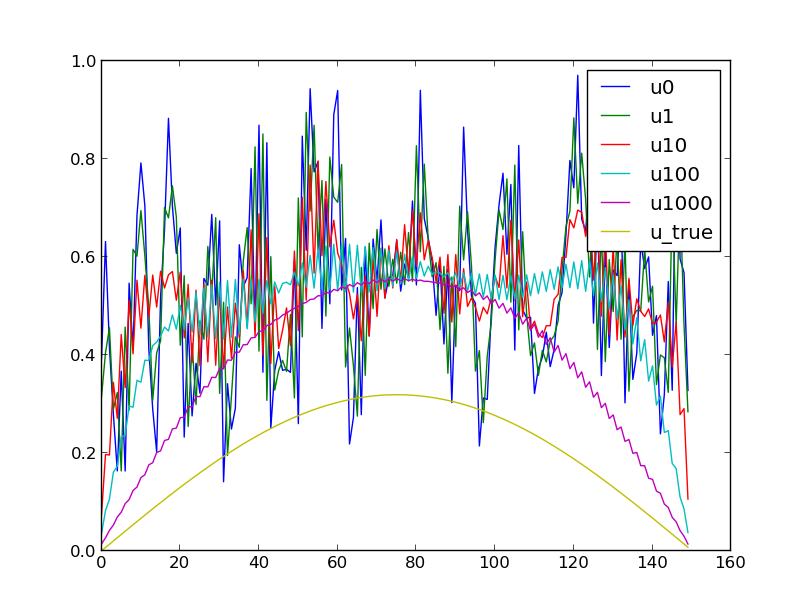
\includegraphics[width=6cm]{../pics/Richardson2.png}
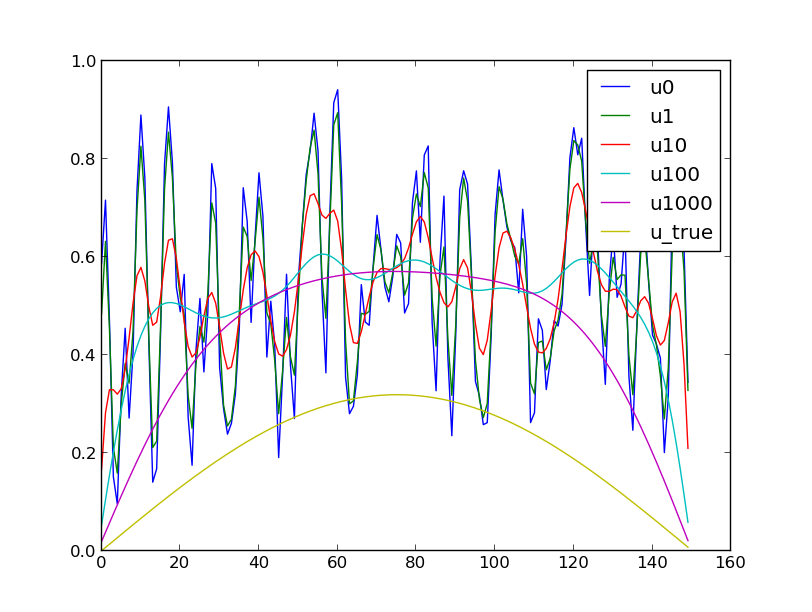
\includegraphics[width=6cm]{../pics/Richardson1.png}
\caption{The numerical solution at different steps of the Richardson method is
shown. The left figure uses
the optimal $\tau$,  that is, $\tau = \frac{2}{\max_i \lambda_i + \|\min_i \lambda_i}$
while $\tau = \frac{0.9}{\max_i \lambda_i}$ is used in the right figure.
}
\end{center}
\end{figure}
Figure \ref{Poisson1D:Rich} show the numerical solution at different iterations when
using the Richardson method for two different $\tau$ values. In both cases
it is clear that the solution improves quite a lot in the first 10 iterations, but
slow down since a large part of the error remain essentially unchanged during the iterations. 
The left figure clearly shows that the solution after 1000 iterations
is dominated by low and high frequency components. The figure on the right,
where $\tau = \frac{0.9}{\max_i \lambda_i}$ shows that the high frequency components
of the error can be removed by choosing a larger than optimal $\tau$.
However, in both cases the low frequency components or the error remains essentially
unchanged throughout the iterations.

The code used in this example is as follows: 
\begin{python}
import numpy

def create_stiffness_matrix(N):
  h = 1.0/(N-1)
  A = numpy.zeros([N,N])
  for i in range(N):
    A[i,i] = 2.0/(h**2)
    if i > 0:
      A[i,i-1] = -1.0/(h**2)
    if i < N-1:
      A[i,i+1] = -1.0/(h**2)
  A = numpy.matrix(A)
  return A

import pylab
from numpy import linalg

N = 150
x = numpy.arange(0, 1, 1.0/(N))
f = numpy.matrix(numpy.sin(3.14*x)).transpose()
u_true = (1.0/3.14)*numpy.matrix(numpy.sin(3.14*x)).transpose()
u0 = numpy.matrix(numpy.random.random(N)).transpose()
u_prev = u0
A = create_stiffness_matrix(N)

eigenvalues = linalg.eigvals(A)
eigenvalues = numpy.sort(eigenvalues)

lambda_max = eigenvalues[-1]

tau = 0.9/lambda_max
for i in range(1001):
  u = u_prev - tau*(A*u_prev - f)
  u_prev = u
  if i == 0 or i == 1 or i == 10 or i == 100 or i == 1000:
    pylab.plot(u)
pylab.plot(u_true)
pylab.legend(["u0", "u1", "u10", "u100", "u1000", "u_true"])
pylab.show()
\end{python}
\end{example}

%\subsection{Some Classical iterations}
%The classical iterations Jacobi, Gauss-Seidel, SOR and SSOR can also be
%written as generalizations of the Richardson iteration. That is, let
%the iteration be
%\[
%u^n = u^{n-1}  - B (f - A u^{n-1}) .
%\]
%The convergence rate
%\[
%\rho = \|I - BA \|,
%\]
%determines the convergence, since
%\[
%e^n = e^{n-1} - B A e^{n-1}.
%\]
%which means that
%\[
%\|e^n\| = \|(I - B A) e^{n-1} \| \le \rho \|e^{n-1} \|  .
%\]
%
%
%
%The convergence of the method would be
%Here we have replaced the previous relaxtion parameter $\tau$ with $B$ which may
%be a matrix or in general a linear operator. Linear operators are operators for
%which we may program algorithms for compting the matrix-vector product $B v$ without
%neccessarily storing or computing the matrix representation.
%
%Let
%\[
%A = D - L - U ,
%\]
%where $D$ is diagonal, $L$ is lower-trianglular, and $U$ is upper-trianglular.
%The  \emph{Jacobi iteration} can be written as
%\begin{equation}
%\label{jacobi}
%u^n = u^{n-1}  - D^{-1} (f - A u^{n-1}) .
%\end{equation}
%and the convergence rate is
%\[
%\rho_{J} = \| I - D^{-1}A \| .
%\]
%The algorithmic expression of the Jacobi iteration is slightly different from \eqref{jacobi}:
%\[
%u^n_i = (f _i -   \sum_{j\not = i} A_{ij} u^{n-1}_j) / A_{ii} .
%\]
%The \emph{Gauss-Seidel iteration} can be written as
%\[
%u^n = u^{n-1}  - (D-L)^{-1} (f - A u^{n-1}) .
%\]
%and the convergence rate is
%\[
%\rho_{GS} = \| I - (D-L)^{-1}A \| .
%\]
%
%The algorithmic expression for the Gauss-Seidel iteration is even more different than for the Jacobi iteration,
%\[
%u^n_i = (f _i -   \sum_{j < i} A_{ij} u^{n}_j  - \sum_{j > i} A_{ij} u^{n-1}_j )  / A_{ii} .
%\]
%
%

\subsection{Order optimal algorithms and Spectral Equivalence}


Any linear iteration for solving the linear system
\[
A u = f,
\]
can be written as
\[
u^n = u^{n-1}  - \tau (f - A u^{n-1}) .
\]
The convergence factor is
\[
\rho = \|I - \tau A \|,
\]
We have also seen that we may introduce a preconditioned system
\[
B A u = B f,
\]
Here, $B$ is a matrix or linear operator designed to make the condition number of the preconditioned system
smaller, while $B$ is cheap (ideally ${\mathcal O} (n)$) in storage and evaluation.
\[
u^n = u^{n-1}  - \tau B (f - A u^{n-1}) .
\]
The convergence factor of the preconditioned iteration is
\[
\rho = \|I - \tau B A \|,
\]


\begin{definition}
Two matrices or linear operators, $B$ and $C$, are spectrally equivalent if
\[
c_0 (B u, u) \le (C u, u) \le c_1 (B u, u), \quad \forall u
\]
The condition number of $B^{-1} C$, $\cond ( B^{-1} C) \le  \frac{c_1}{c_0} $.
\end{definition}


Hence a spectral equivalent preconditioner guaranties a convergence rate
independent of the mesh resolution and therefore an order optimal algorithm, since $\ldots$.




\section{Krylov methods and preconditioning}

Any linear iteration may be written as a Richardson iteration with a preconditioner.
However, iterations like Conjugate Gradient method, GMRES, Mininal Residual method, and
BiCGStab, are different. These are non-linear iterations methods. We will not 
go in detail on these methods, but they should be used together with a
preconditioner, just as Richardson. Furthmore, some of then have special requirements.   

\paragraph{Classification of methods}
We classify the methods according to the matrices they solve
The matrix may be:
\begin{itemize}
\item Symmetric Positive Definite: use Conjugate Gradient with an SPD preconditioner, see also Exercise \ref{ex:poisson}. 
\item Symmetric and indefinite: use Minimal Residual method with and SPD preconditioner, see also Exercise \ref{ex:stokes}.  
\item Positive: GMRES and ILU (or AMG) is often good, but you might need to experiment, see also Exercise \ref{ex:conv}. 
\item Nonsymmetric and indefinite: all bets are off. 
\end{itemize}



%\section{The Multigrid method}
%\section{The Domain decomposition method}


\begin{exercise}
Implement the Richardson iteration for the 1D Poisson problem with homogenous
Dirichlet conditions, using finite differences and a multigrid preconditioner. 
\end{exercise}

\begin{exercise}
Estimate the convergence factor for the Jacobi and Gauss-Seidel iteration for the 1D Poisson problem from Example \ref{ex1}.
\end{exercise}

\begin{exercise}
\label{ex:poisson}
Test CG method with no, ILU and AMG preconditioner for the Poisson problem in 1D and 2D with
homogenous Dirichlet conditions,  with respect
to different mesh resolutions. Do some of the iterations suggest spectral equivalence?
\end{exercise}

\begin{exercise}
\label{ex:conv}
Test CG, BiCGStab, GMRES with ILU, AMG, and Jacobi preconditioning for 
\begin{eqnarray*}
-\mu\Delta u + v\nabla u   &=& f \quad \textrm{in}\ \Omega\\
u&=& 0 \quad \textrm{on}\ \partial\Omega
\end{eqnarray*}
Here $\Omega$ is the unit square, $v=c sin(7 x)$, and $c$ varies as $1, 10, 100, 1000, 10 000$ and
the mesh resolution $h$ varies as $1/8, 1/16, 1/32, 1/64$. You may assume homogenous Dirichlet conditions.  

\end{exercise}

\begin{exercise}
\label{ex:stokes}
The following code snippet shows the assembly of the matrix and preconditioner
for a Stokes problem: 
\begin{python} 
a = inner(grad(u), grad(v))*dx + div(v)*p*dx + q*div(u)*dx
L = inner(f, v)*dx

# Form for use in constructing preconditioner matrix
b = inner(grad(u), grad(v))*dx + p*q*dx

# Assemble system
A, bb = assemble_system(a, L, bcs)

# Assemble preconditioner system
P, btmp = assemble_system(b, L, bcs)

# Create Krylov solver and AMG preconditioner
solver = KrylovSolver("tfqmr", "amg")

# Associate operator (A) and preconditioner matrix (P)
solver.set_operators(A, P)

# Solve
U = Function(W)
solver.solve(U.vector(), bb)
\end{python} 
Here, "tfqmr" is a variant of the Minimal residual method and "amg" is an algebraic 
multigrid implementation in HYPRE. Test, by varying the mesh resolution, whether
the code produces an order--optimal preconditioner.  
HINT: You might want to change the "parameters" as done
in Example \ref{ex1}: 
\begin{python}
# Create Krylov solver and AMG preconditioner
solver = KrylovSolver("tfqmr", "amg")
solver.parameters["relative_tolerance"] = 1.0e-8
solver.parameters["absolute_tolerance"] = 1.0e-8
solver.parameters["monitor_convergence"] = True
solver.parameters["report"] = True
solver.parameters["maximum_iterations"] = 50000
\end{python}
\end{exercise}


\end{document}


